\documentclass{article}
\usepackage[utf8]{inputenc}
\usepackage{amsmath}
\usepackage{booktabs}
\usepackage{float}
\usepackage{subcaption}
\usepackage{graphicx}
\usepackage[top=1in, bottom=1.25in, left=1.25in, right=1.25in]{geometry}

\title{Enzyme Kinetics Analysis Report}
\author{Jozef Fülöp}
\date{March 2023}

\begin{document}

\maketitle

\section{Introduction}
Enzyme kinetics is the study of the chemical
reactions that are catalyzed by enzymes.
This report analyzes two sets of experimental data on enzyme kinetics,
one with an inhibitor and one without an inhibitor.
Calculates the $V_{max}$, $K_M$ and $K_I$ values.

\section{Input data}

\begin{table}[htbp]
    \centering
    \begin{subtable}{\textwidth}
        \centering
        \caption{Reaction without inhibitor}
        \begin{tabular}{cccc}
            \hline
            [S](mmol/l) & [I](mmol/l) & V (µmol/L/min) \\
            \hline
            1           & 0           & 0.67           \\
            2           & 0           & 1.13           \\
            3           & 0           & 1.48           \\
            4           & 0           & 1.74           \\
            5           & 0           & 1.98           \\
            \hline
        \end{tabular}
    \end{subtable}
    \begin{subtable}{\textwidth}
        \centering
        \caption{Reaction with inhibitor}
        \begin{tabular}{cccc}
            \hline
            [S](mmol/l) & [I](mmol/l) & V (µmol/L/min) \\
            \hline
            1           & 1           & 0.05           \\
            2           & 1           & 0.10           \\
            3           & 1           & 0.15           \\
            4           & 1           & 0.16           \\
            5           & 1           & 0.18           \\
            \hline
        \end{tabular}
    \end{subtable}
    \caption{Reaction rates with and without inhibitor}
\end{table}

\subsection*{Equations}

The Michaelis-Menten equation is given by:
\begin{equation}
    V = V_{max} \frac{[S]}{K_{M} + [S]}
\end{equation}

The Lineweaver-Burk equation is given by:
\begin{equation}
    \frac{1}{V} = \frac{1}{V_{max}} + \frac{1}{K_{M}} \cdot \frac{1}{[S]}
\end{equation}

The Michaelis-Menten equation can be derived from the Lineweaver-Burk equation by
multiplying both sides by $V$ and rearranging the terms:
\begin{equation}
    V = \frac{V_{max}}{\displaystyle 1 + \frac{K_{M}}{[S]}}
\end{equation}

The Michaelis-Menten equation can be used to calculate the $K_I$ value, in noncompetitive
inhibition, as follows: % V = ((Vmax / (1 + [I]/Ki)) * [S]) / (Km + [S])
\begin{equation}
    V = \frac{\displaystyle \frac{V_{max}}{1 + \frac{[I]}{K_{I}}} \cdot [S]}{K_{M} + [S]}
\end{equation}

\subsection*{Plots}

\begin{figure}[H]
    \centering
    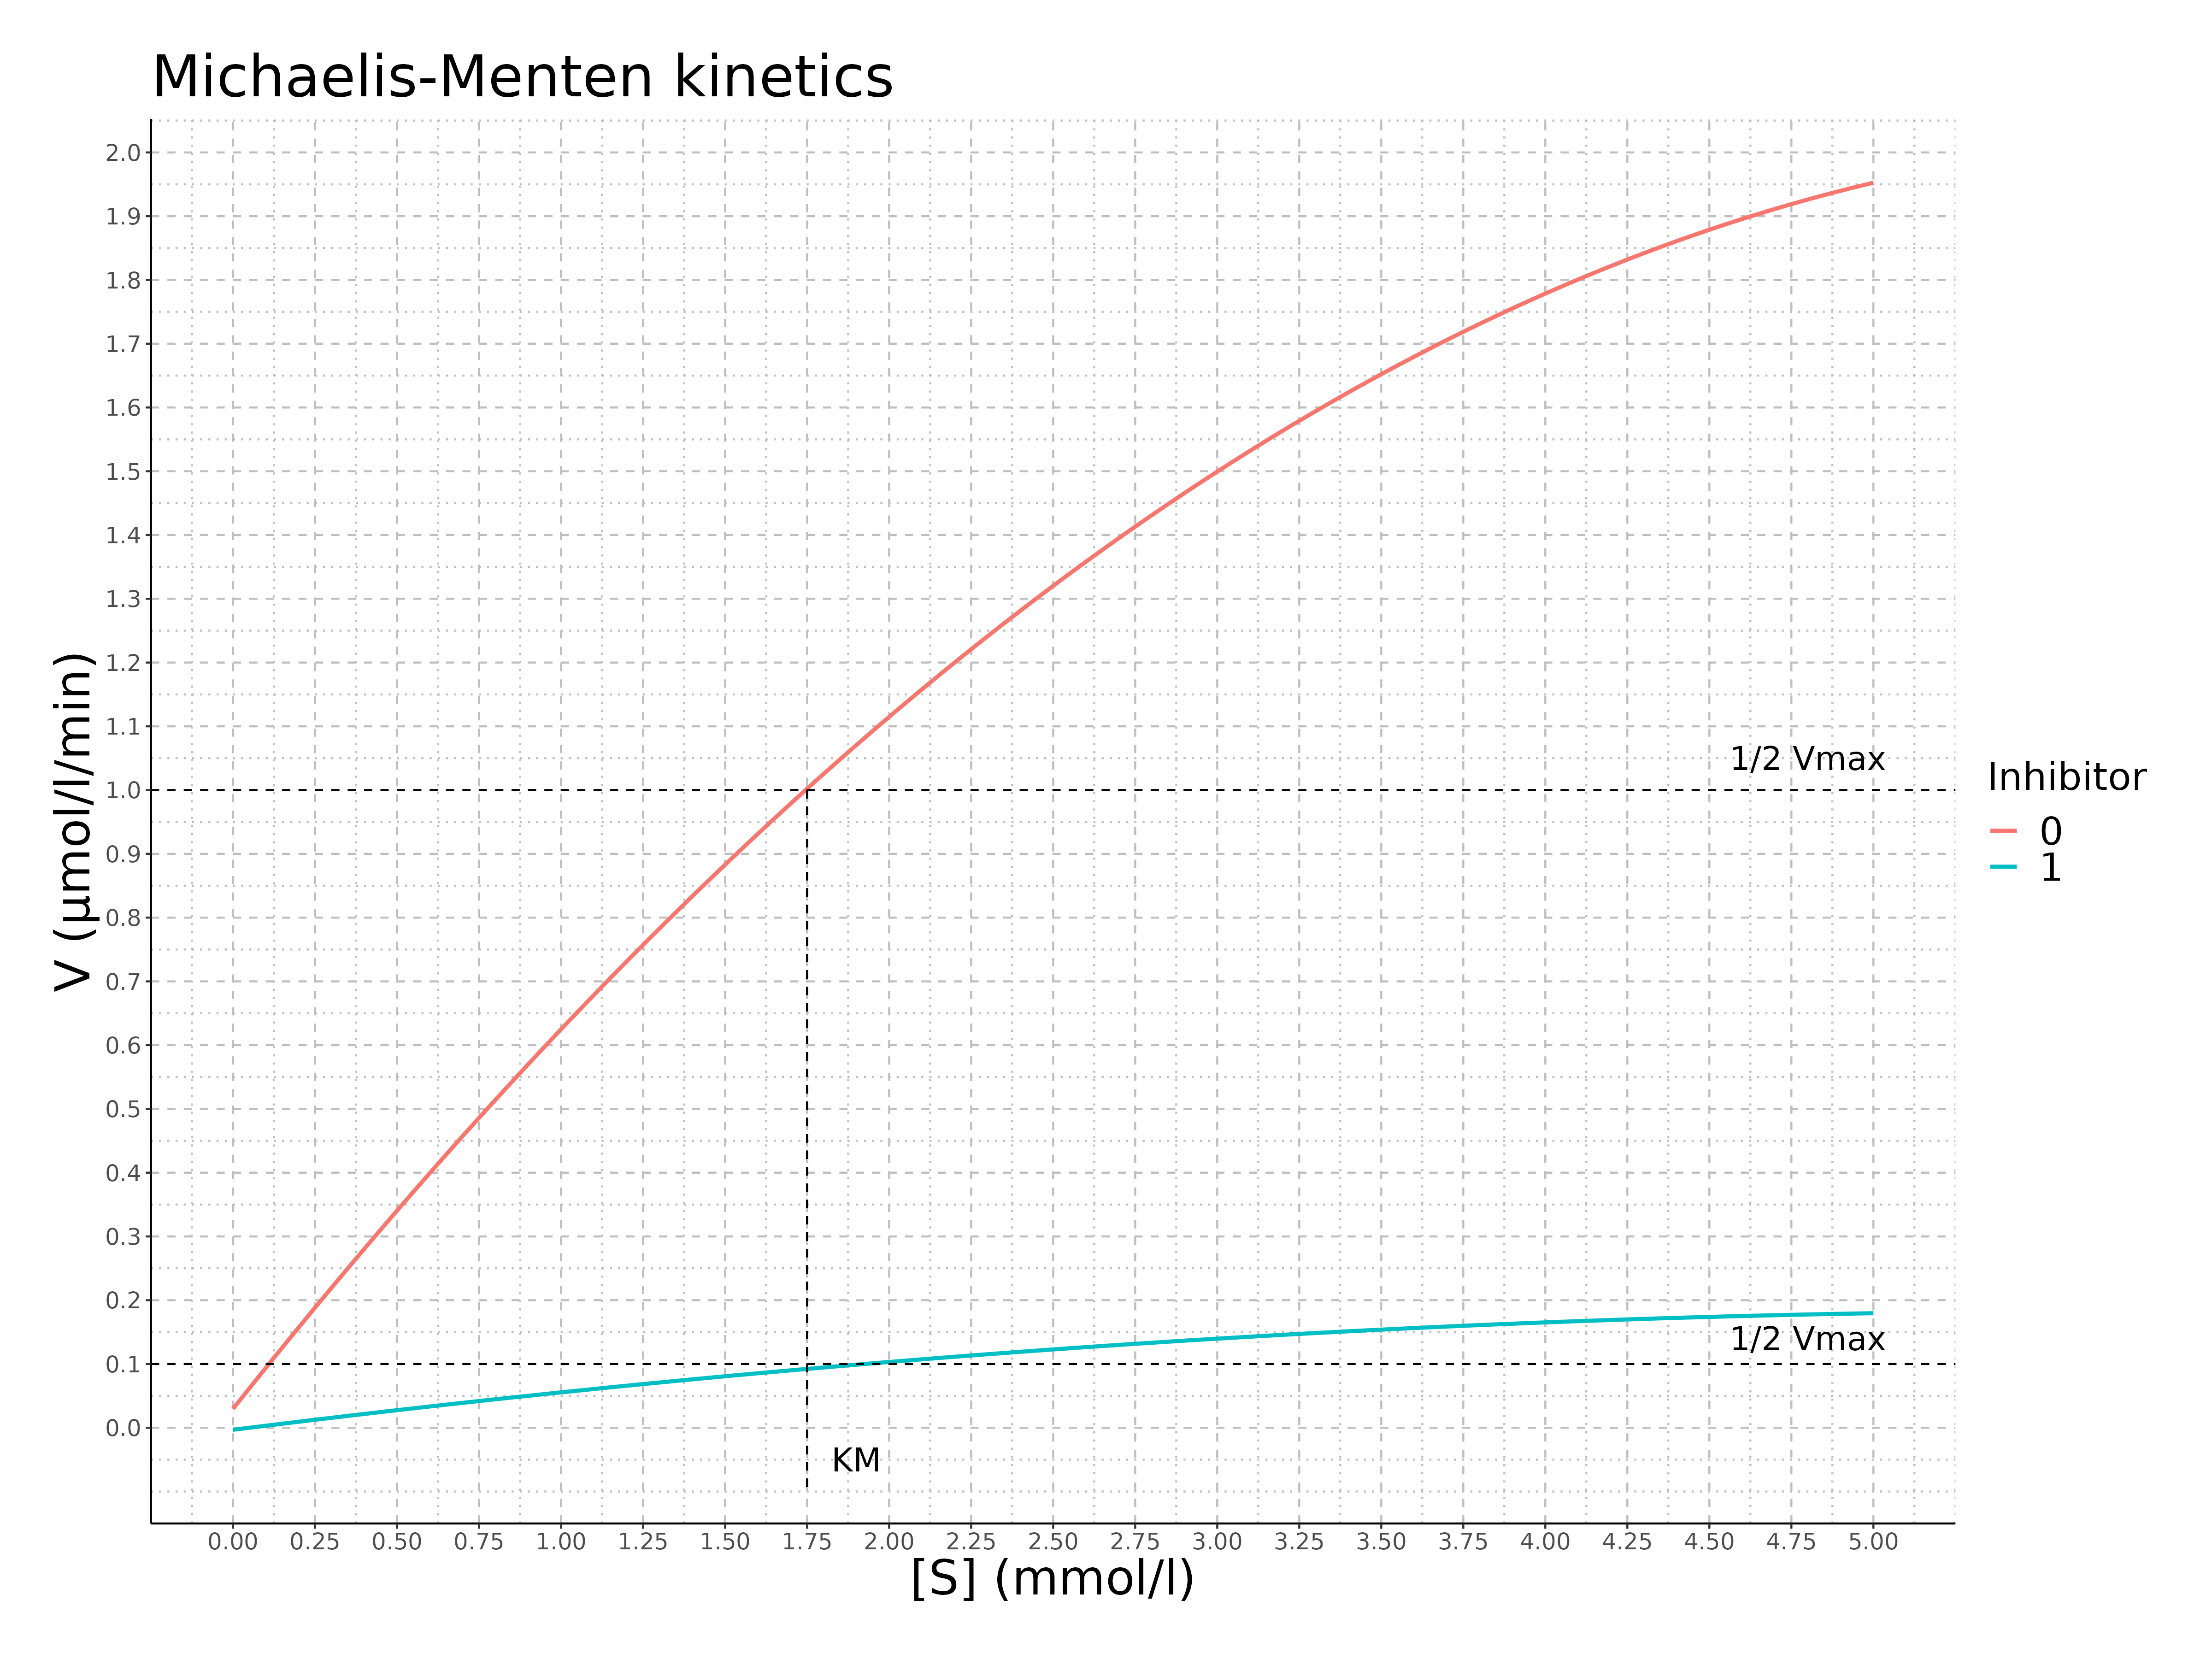
\includegraphics[width=1.0\textwidth, height=0.5\textheight]{plots/data_plot1.png}
    \caption{Michaelis-Menten kinetics plot showing the relationship
        between substrate concentration and reaction rate with and without inhibitor.
        The plot also includes fitted values and 1/2 $V_{max}$ lines for both datasets.}
    \label{fig:MMplot}
\end{figure}


\begin{figure}[H]
    \centering
    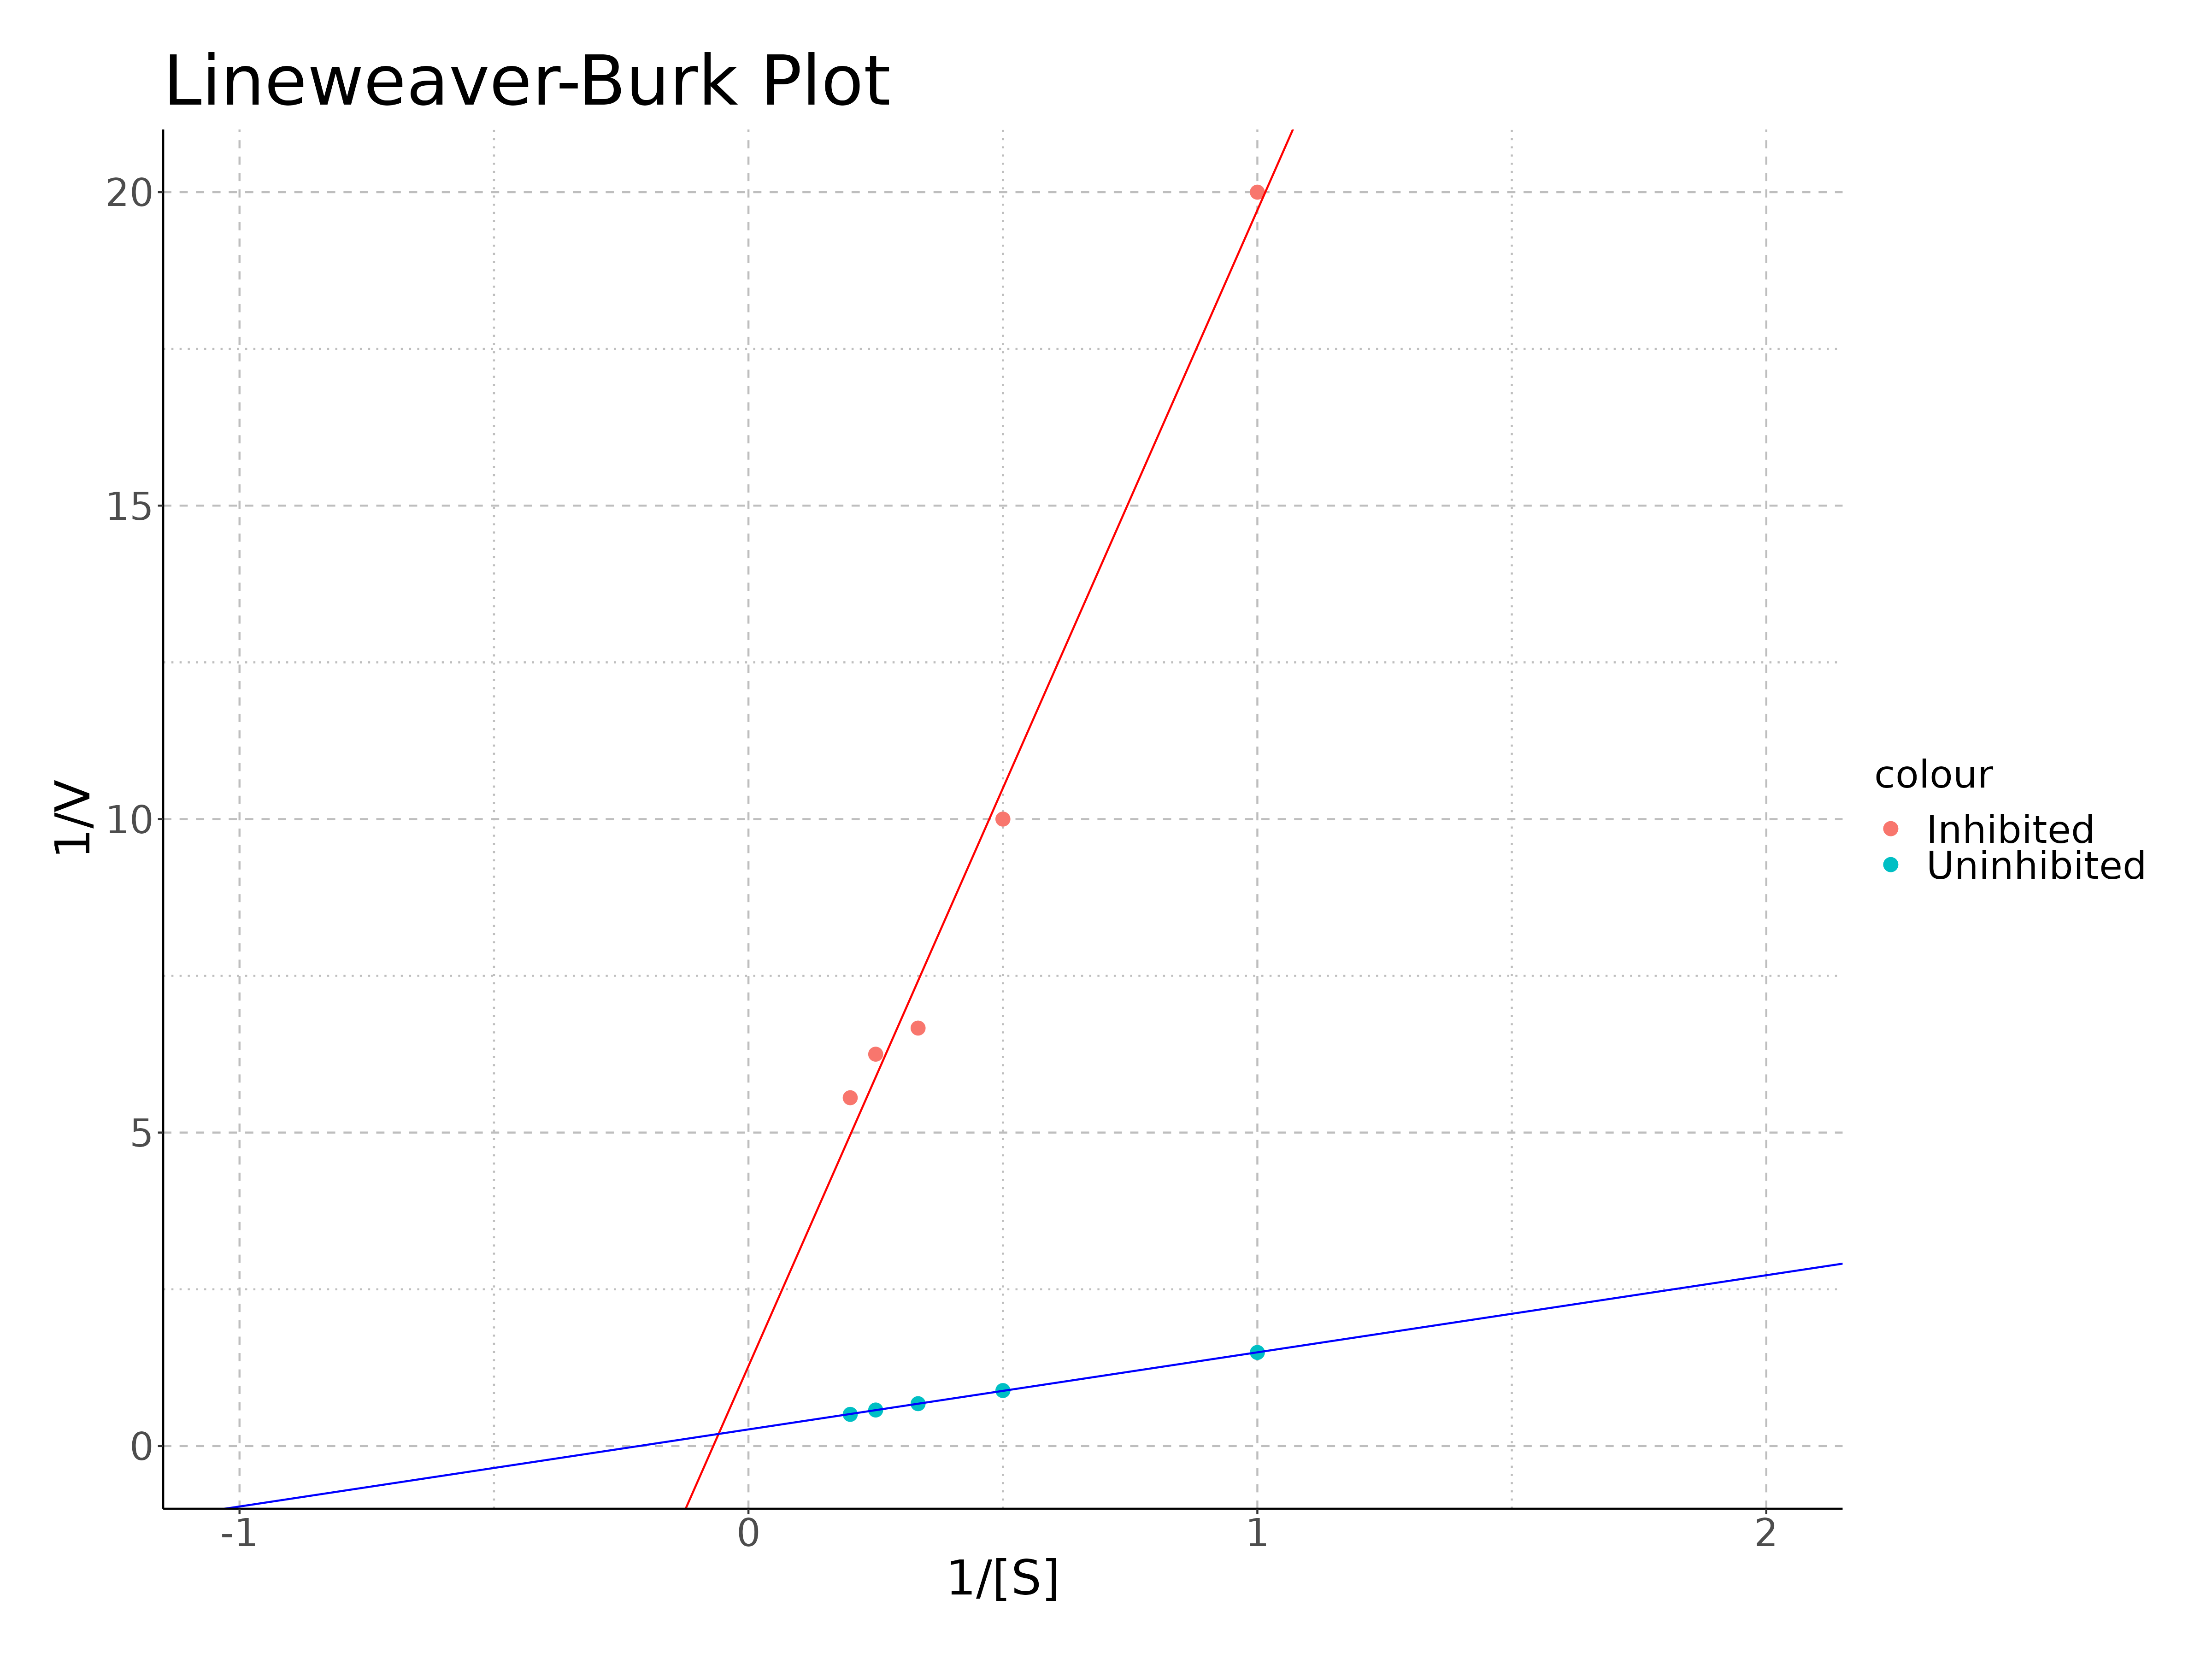
\includegraphics[width=1.0\textwidth, height=0.5\textheight]{plots/Lineweaver-Burk_big.png}
    \caption{Lineweaver-Burk plot showing the reciprocal of substrate concentration
    ($1/[S]$) versus the reciprocal of enzyme velocity ($1/V$) for inhibited (red) and
    uninhibited (blue) enzyme reactions. The plot includes two linear regression lines with
    slopes and intercepts calculated from the data.}

    \label{fig:lineweaver-burk}
\end{figure}

\section{Uninhibited Reaction}

The first set of data is from an uninhibited reaction. The data was fit to the
Michaelis-Menten equation $V = V_{max} \displaystyle \frac{[S]}{K_{M} + [S]}$, where $V_{max}$ is the
maximum velocity of the reaction, $[S]$ is the substrate concentration, and $K_{M}$ is the
Michaelis constant. The fitted parameters are as follows:
\begin{itemize}
    \item $V_{max}$ = 3.89 $\pm$ 0.08 mmol/l
    \item $K_{M}$ = 4.88 $\pm$ 0.18 µmol/L/min
\end{itemize}

\begin{table}[H]
    \caption{Model summary without inhibitor}
    \centering
    \begin{tabular}[t]{l|r|r|r|r}
        \hline
                  & Estimate & Std. Error & t value  & Pr($>|t|$) \\
        \hline
        $V_{max}$ & 3.892276 & 0.0846582  & 45.97636 & 0.0000227  \\
        \hline
        $K_{M}$   & 4.881717 & 0.1828702  & 26.69498 & 0.0001153  \\
        \hline
    \end{tabular}
\end{table}

\begin{table}[H]

    \caption{Confidence interval for Vm and Km for uninhibited reaction}
    \centering
    \begin{tabular}[t]{l|r|r}
        \hline
                  & 2.5\%    & 97.5\%   \\
        \hline
        $V_{max}$ & 3.640811 & 4.185819 \\
        \hline
        $K_{M}$   & 4.340821 & 5.518560 \\
        \hline
    \end{tabular}
\end{table}

\section{Inhibited Reaction}

The second set of data is from an inhibited reaction. The data was fit to the Michaelis-Menten
equation $V = V_{max}\displaystyle \frac{[S]}{K_{M} + [S]}$, where $V_{max}$ is the maximum velocity of the
reaction, $[S]$ is the substrate concentration, and $K_{M}$ is the Michaelis constant. The
fitted parameters are as follows:
\begin{itemize}
    \item $V_{max}$ = 0.39 $\pm$ 0.10 mmol/l
    \item $K_{M}$ = 5.71 $\pm$ 2.30 µmol/L/min
\end{itemize}

\begin{table}[H]

    \caption{Model summary with inhibitor}
    \centering
    \begin{tabular}[t]{l|r|r|r|r}
        \hline
                  & Estimate  & Std. Error & t value  & Pr($>|t|$) \\
        \hline
        $V_{max}$ & 0.3945488 & 0.0974732  & 4.047765 & 0.0271504  \\
        \hline
        $K_{M}$   & 5.7125880 & 2.2981536  & 2.485729 & 0.0888187  \\
        \hline
    \end{tabular}
\end{table}

\begin{table}[H]

    \caption{Confidence interval for $V_{max}$ and $K_{M}$ for inhibited reaction}
    \centering
    \begin{tabular}[t]{l|r|r}
        \hline
                  & 2.5\%     & 97.5\%    \\
        \hline
        $V_{max}$ & 0.2437008 & 3.270304  \\
        \hline
        $K_{M}$   & 2.5583919 & 74.920253 \\
        \hline
    \end{tabular}
\end{table}

\begin{figure}[H]
    \centering
    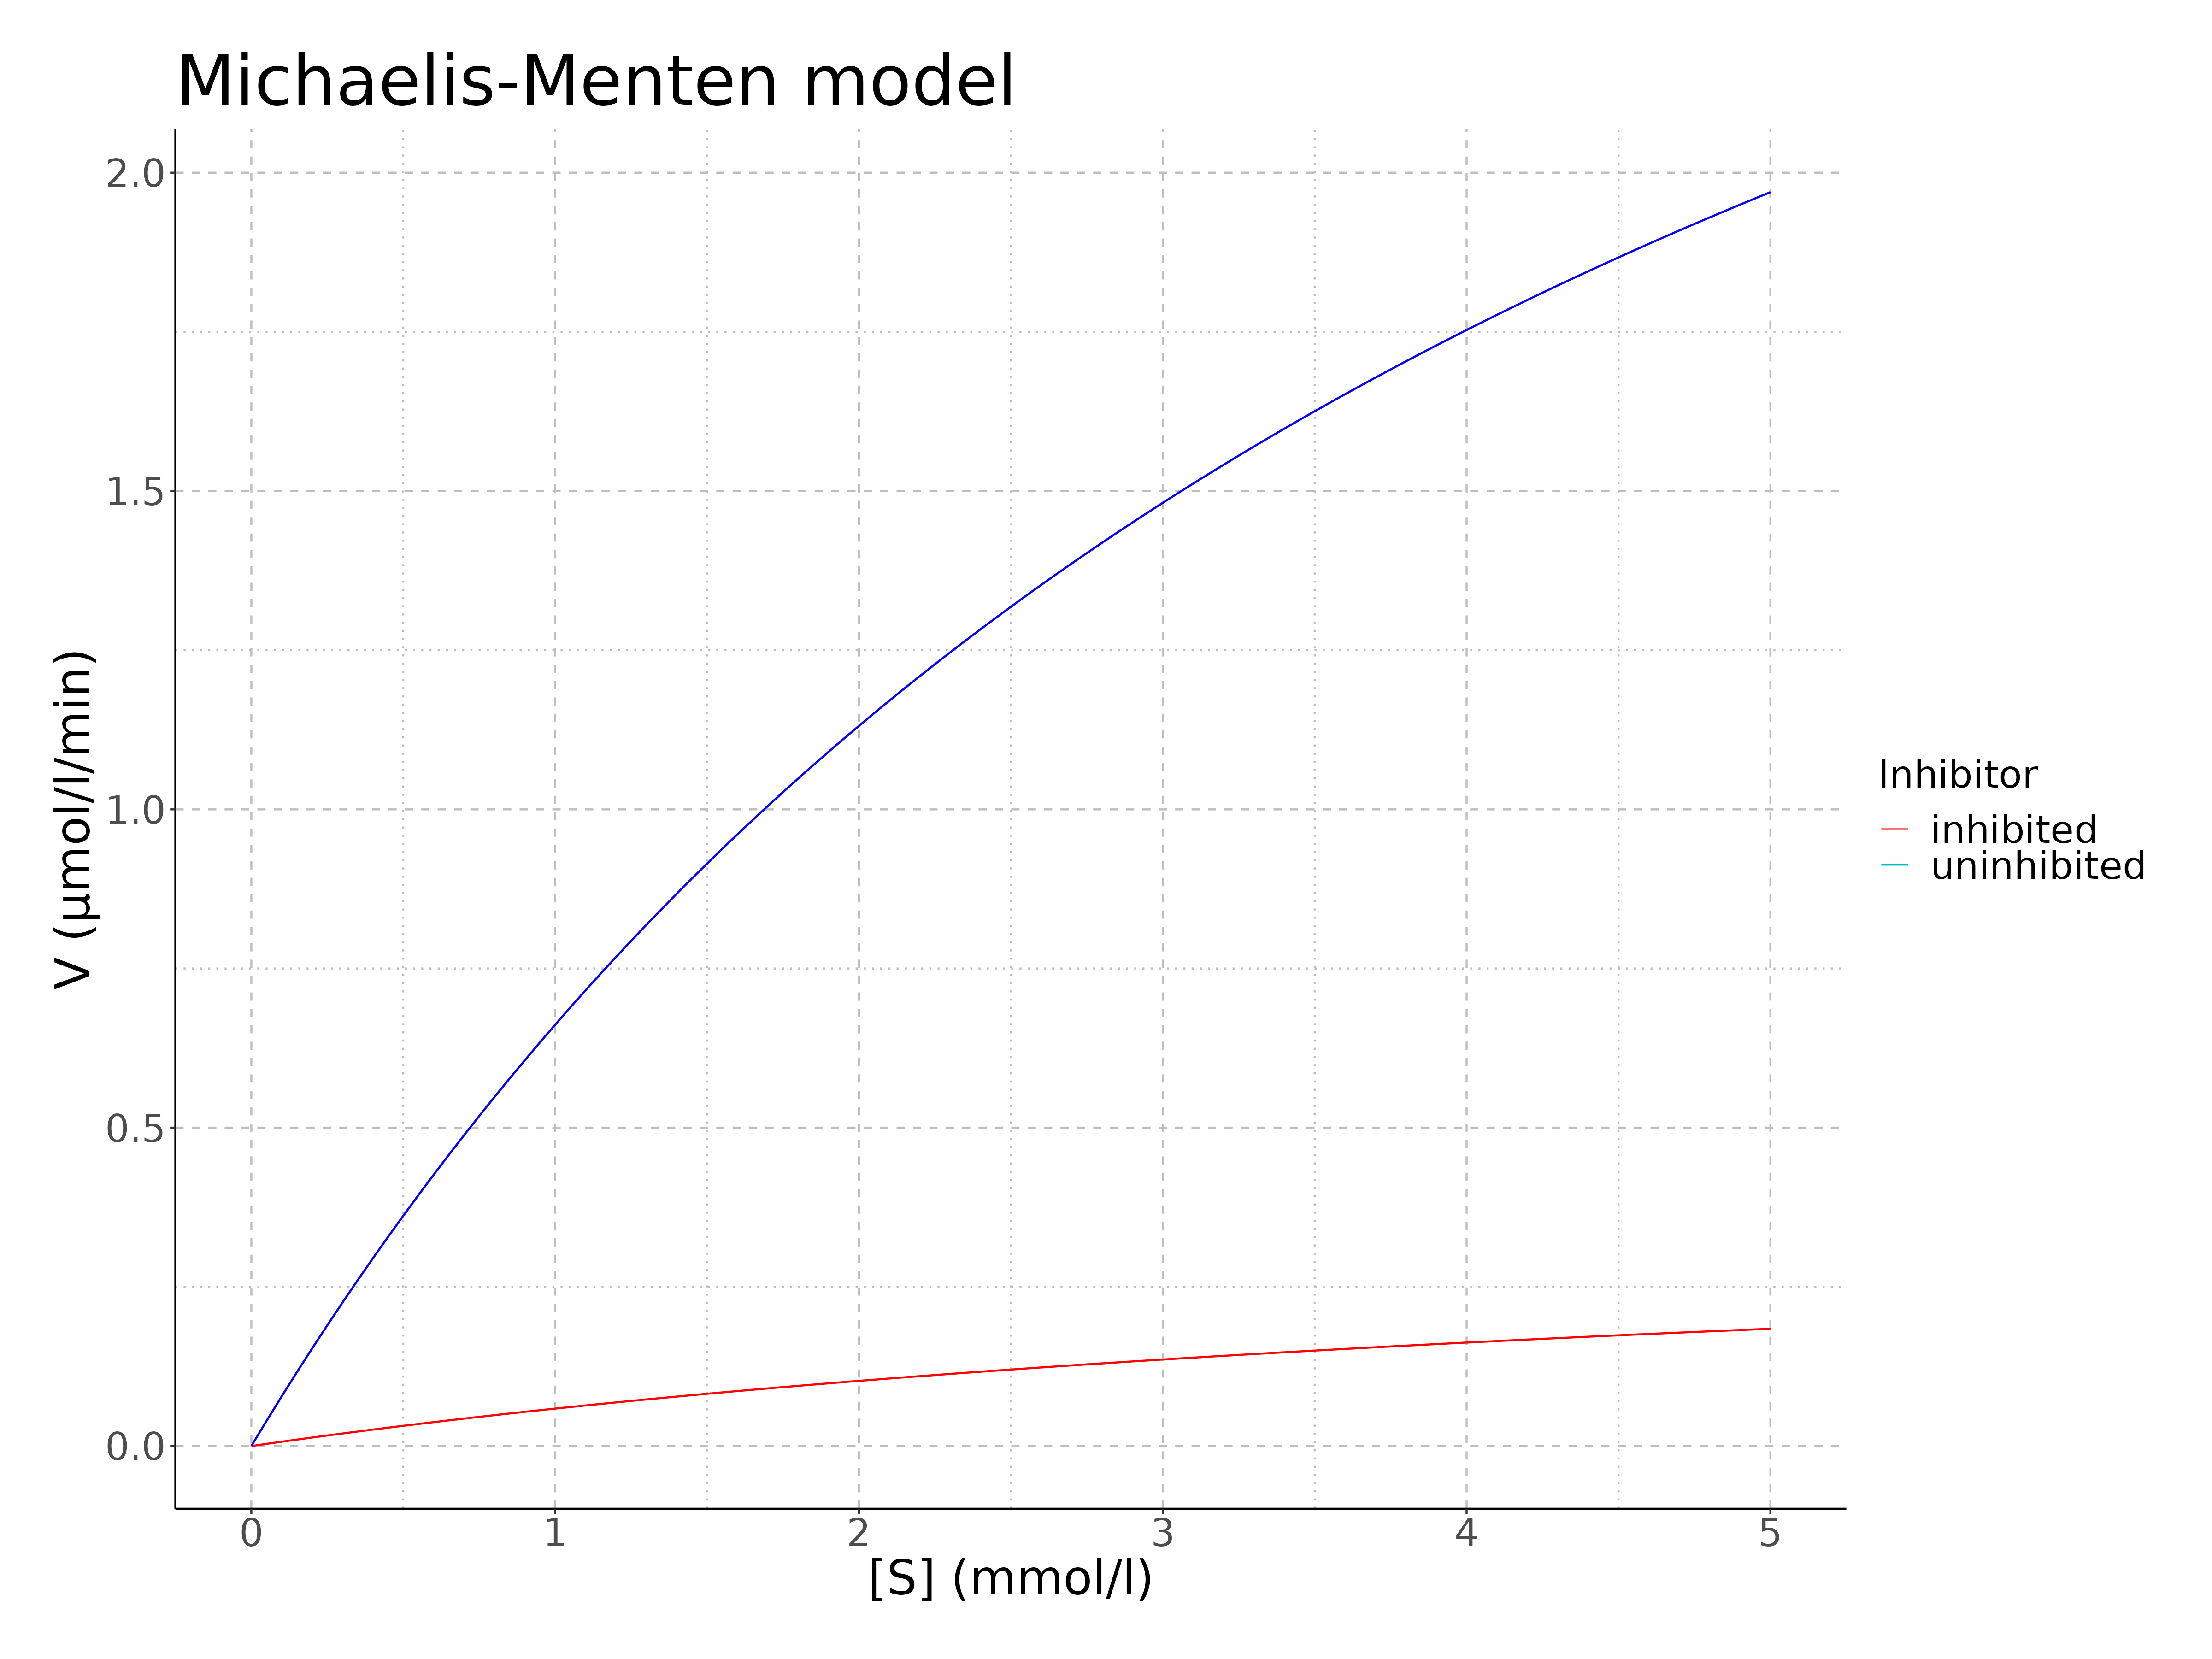
\includegraphics[width=1.0\textwidth, height=0.5\textheight]{plots/model_fit_plot2.png}
    \caption{Michaelis-Menten model for enzyme kinetics, showing the substrate concentration [S] (mmol/l)
        on the x-axis and the reaction rate V (µmol/l/min) on the y-axis. The blue line represents the reaction
        rate without inhibitor, while the red line shows the reaction rate with inhibitor. The legend indicates
        whether the inhibitor is present or absent. The plot illustrates the effect of an inhibitor on the enzyme
        activity, with the inhibited reaction rate curve shifted downwards compared to the uninhibited reaction rate curve.}
    \label{fig:enzyme_kinetics}
\end{figure}

\section{Non-competitive inhibition}

The data was fit to the same Michaelis-Menten equation as before, but with an additional term to account for
the inhibitor: $    V =\displaystyle \frac{\displaystyle \frac{V_{max}}{1 + \frac{[I]}{K_{I}}} \cdot [S]}{K_{M} + [S]}
$\\ where $[I]$ is the inhibitor
concentration and $K_{I}$ is the inhibition constant. The fitted parameters are as follows:
\begin{itemize}
    \item $V_{max}$ = 0.39 $\pm$ 0.10 µmol/L/min
    \item $K_{M}$ = 5.71 $\pm$ 2.30 mmol/l
    \item $K_{I}$ = 0.10 $\pm$ 0.00 mmol/l
\end{itemize}

\begin{table}[H]

    \caption{Model summary for non-competitive inhibition}
    \centering
    \begin{tabular}[t]{l|r|r|r|r}
        \hline
                  & Estimate  & Std. Error & t value  & Pr($>|t|$) \\
        \hline
        $V_{max}$ & 3.8955119 & 0.0767059  & 50.78505 & 0          \\
        \hline
        $K_{M}$   & 4.8887879 & 0.1656901  & 29.50562 & 0          \\
        \hline
        $K_{I}$   & 0.1017605 & 0.0036314  & 28.02254 & 0          \\
        \hline
    \end{tabular}
\end{table}

\begin{table}[H]

    \caption{Confidence interval for non-competitive inhibition}
    \centering
    \begin{tabular}[t]{l|r|r}
        \hline
                  & 2.5\%     & 97.5\%    \\
        \hline
        $V_{max}$ & 3.7222470 & 4.0877450 \\
        \hline
        $K_{M}$   & 4.5155594 & 5.3052748 \\
        \hline
        $K_{I}$   & 0.0932454 & 0.1104207 \\
        \hline
    \end{tabular}
\end{table}

\begin{figure}[H]
    \centering
    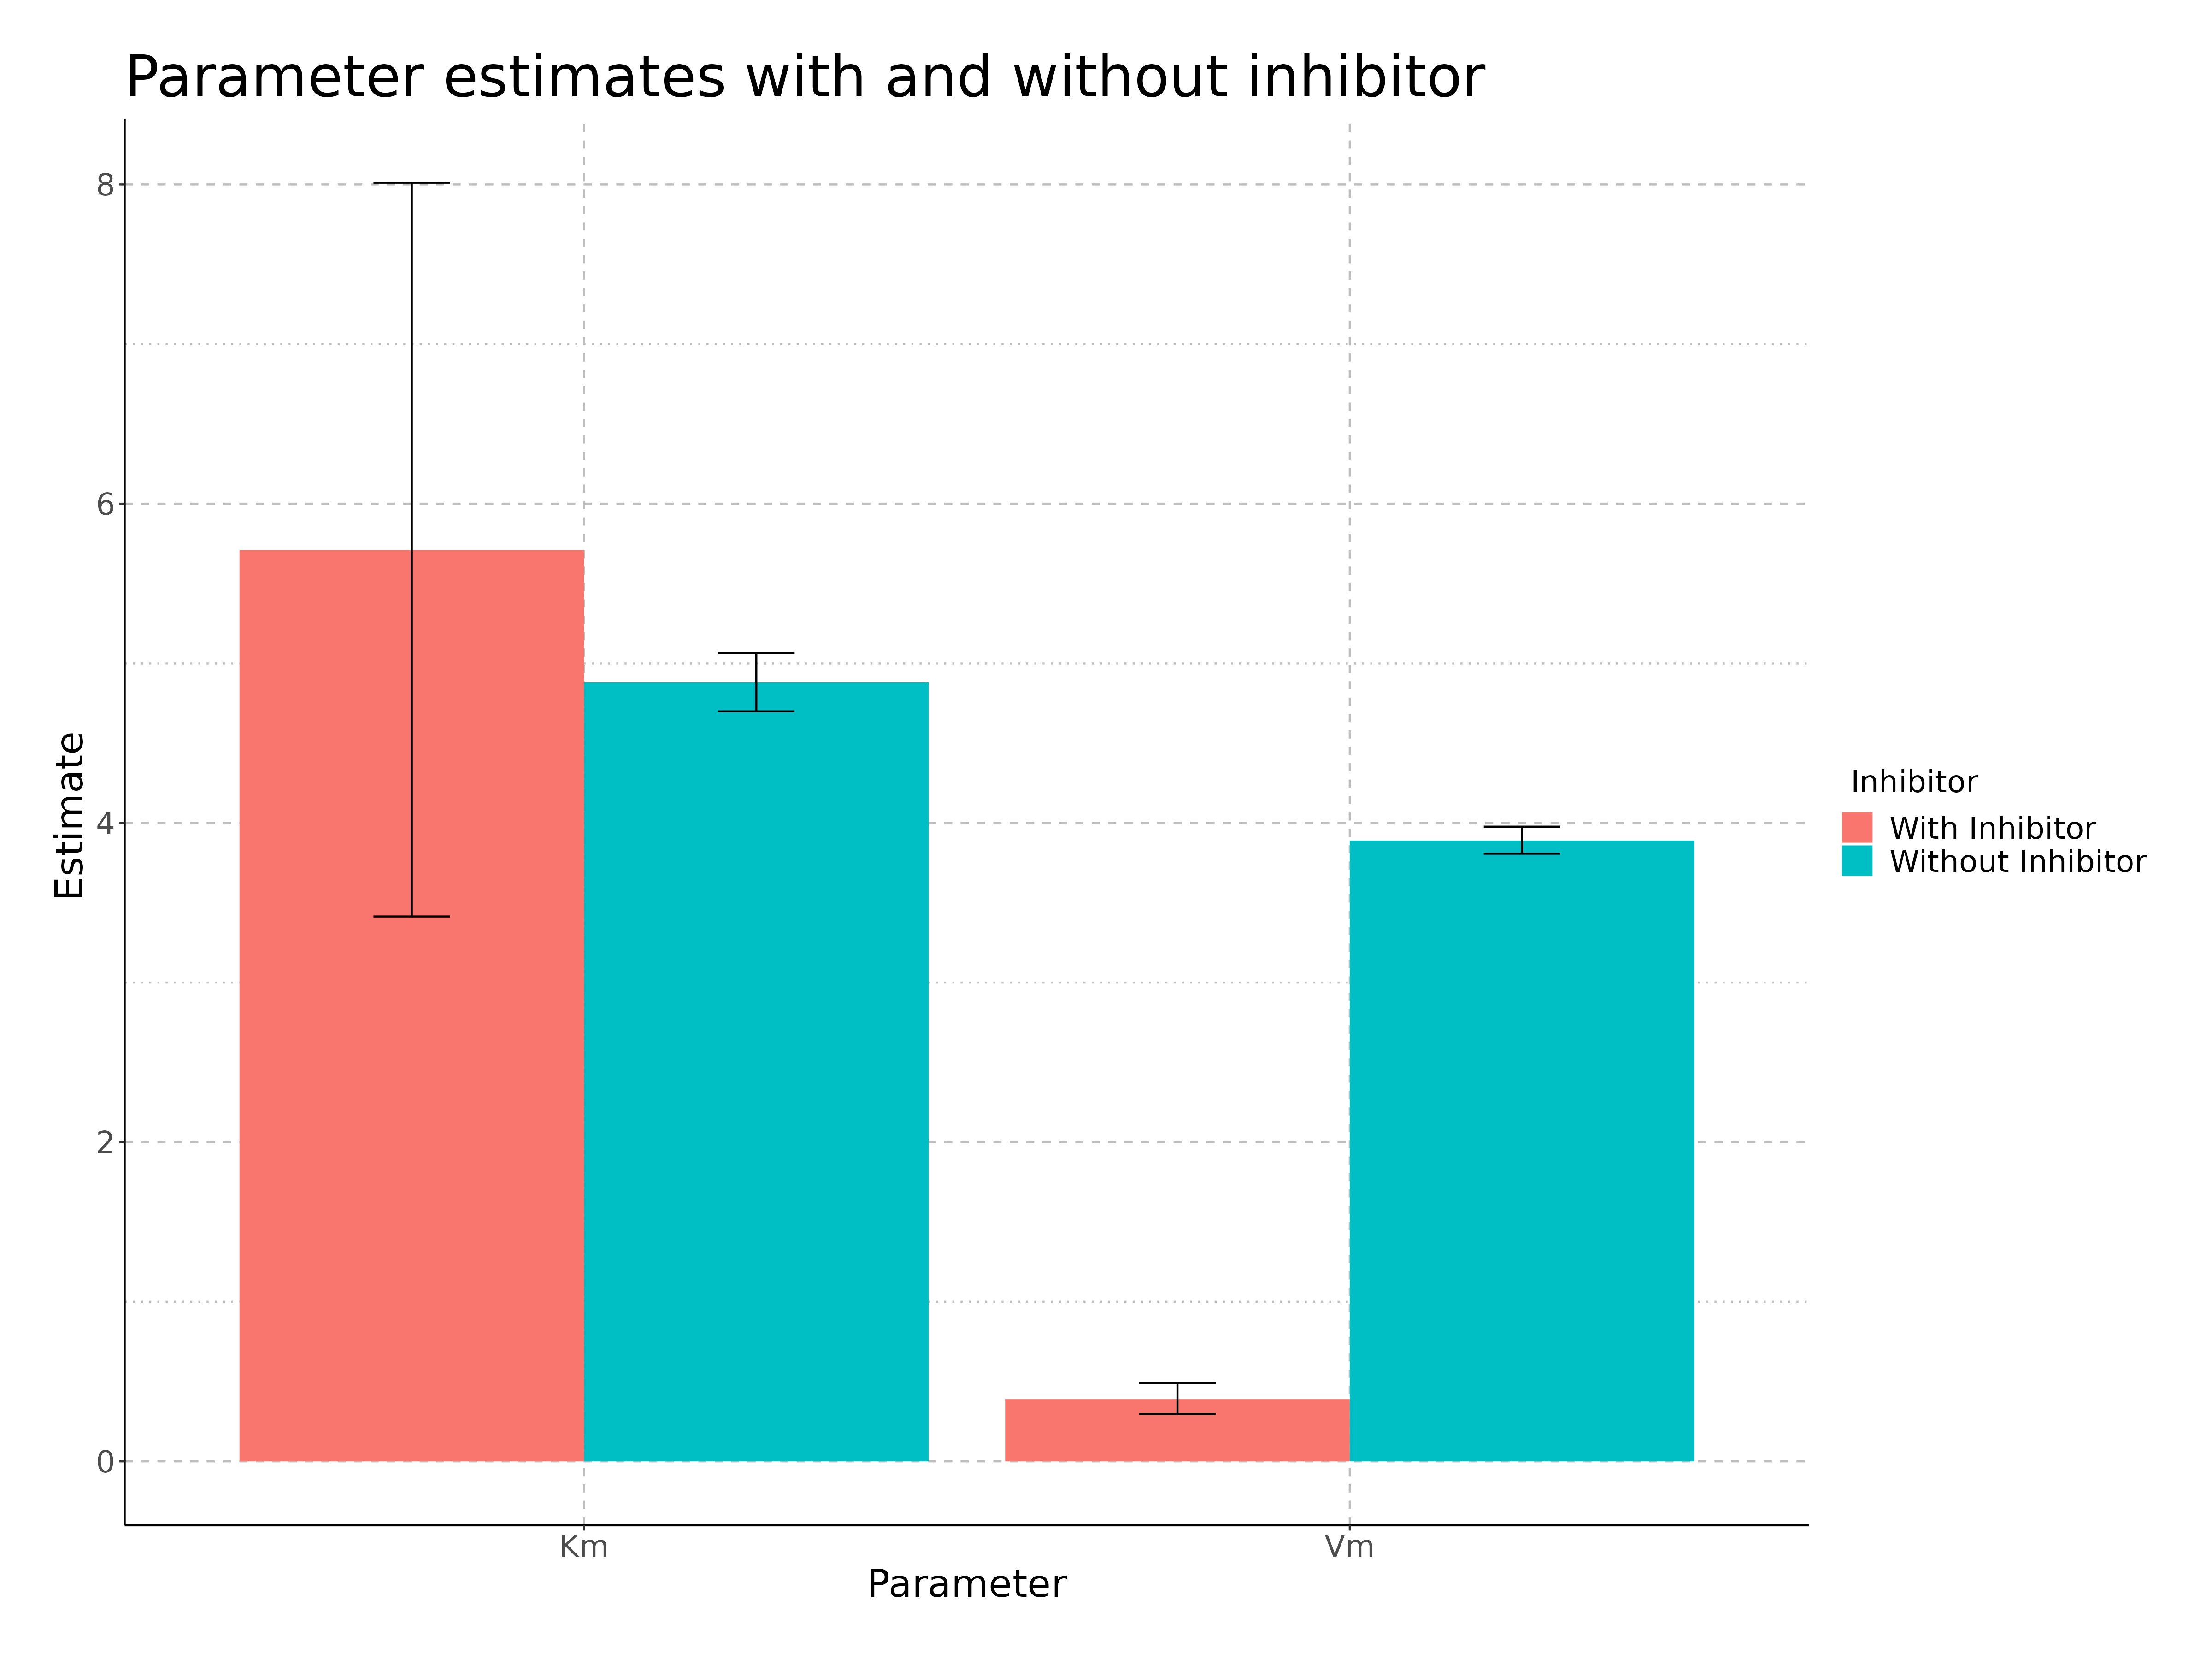
\includegraphics[width=1.2\textwidth, height=0.5\textheight]{plots/enzyme_hw_plot3.png}
    \caption{Bar plot showing parameter estimates with and without inhibitor for the $V_{max}$ and $K_M$ parameters.
        Error bars represent the standard error of the estimates.}
    \label{fig:Bar plot $V_{max}$ $K_{M}$}
\end{figure}

\section{Discussion}
% to do - discuss the results

% add url to github repo
\section{Code}
The code for this project can be found at \url{https://github.com/dodes24/enzymology}\\
Code was written in R and jupyter notebook was used to create the project.
Latex was used to create the report.

\end{document}